\documentclass[12pt,a4paper]{article}
\usepackage[utf8]{inputenc}
\usepackage[T1]{fontenc}
\usepackage{lipsum}% juste utile ici pour générer du faux texte}
\usepackage{amsmath,amsfonts,amssymb}%extensions de l'ams pour les mathématiques
\usepackage{graphicx}%pour insérer images et pdf entre autres
\usepackage[left=3cm,right=2cm,top=1.5cm,bottom=2.5cm]{geometry}%réglages des marges du document selon vos préférences ou celles de votre établissement
\usepackage[english]{babel}%pour un document en français
\usepackage{vmargin}
\usepackage{enumitem}
\usepackage[verbose]{wrapfig}
\usepackage{endnotes}
\usepackage{tikz}
\usepackage{hyperref}
\usepackage{float}
\usepackage{textcomp} 
\usepackage{array,multirow,makecell}
\setcellgapes{1pt}
\makegapedcells
\usepackage{lscape}
\usepackage{caption}
\usepackage{subcaption}
\usepackage{graphicx}
\usepackage{afterpage}
\usepackage{mathtools}
\usepackage{amsmath,siunitx}

\usepackage{listings}
\usepackage[framemethod=default]{mdframed}
\usepackage{adjustbox}

%\usepackage[backend=bibtex]{biblatex}
\usepackage[resetlabels,labeled]{multibib}

\numberwithin{equation}{section}
\everymath{\displaystyle}

\begin{document}

\newenvironment{changemargin}[2]{\begin{list}{}{%
\setlength{\topsep}{0pt}%
\setlength{\leftmargin}{0pt}%
\setlength{\rightmargin}{0pt}%
\setlength{\listparindent}{\parindent}%
\setlength{\itemindent}{\parindent}%
\setlength{\parsep}{0pt plus 1pt}%
\addtolength{\leftmargin}{#1}%
\addtolength{\rightmargin}{#2}%
}\item }{\end{list}}

% définition de la taille de la feuille
\headsep 0.0cm
\textheight=23cm
\textwidth=16.8cm
\hoffset=0.0cm
\oddsidemargin 0cm
\evensidemargin 0cm
\voffset=0.5cm
\topmargin 0cm
\headheight 0.5cm

%%%%%%%%%%%%%%%%%%%%%%%%%%%%%%%%%%%%%%%%%%%%%%%%%%%%%%%%%%%%%%%%%%%%%%
\begin{titlepage}
\begin{center}
\newcommand{\HRule}{\rule{\linewidth}{0.5mm}}

\vspace*{1cm}
\textsc{\LARGE Sorbonne Université}

\begin{center} 
{Erasmus student - Master level}
\end{center}
\vspace*{1cm}
\begin{center}

\includegraphics[width=0.25\textwidth]{Logo.png}
\end{center}
\HRule \\[0.4cm]
{ \huge \bfseries Hyper-elastic laws in a 1D model of an artery\\[0.4cm] }
\HRule \\[1.5cm]
\begin{center} 
{Elisa Ghiringhelli}
\end{center}
\vspace*{1cm}
\vspace*{7cm}
% Author and supervisor

\begin{minipage}{0.4\textwidth}
\begin{flushleft} \large
\emph{Année universitaire 2017-2018}
\end{flushleft}
\end{minipage}

\end{center}

\end{titlepage}
%%%%%%%%%%%%%%%%%%%%%%%%%%%%%%%%%%%%%%%%%%%%%%%%%%%%%%%%%%%%%%%%%%%%%%
\newpage
\tableofcontents

\newpage

\section*{Introduction}
\addcontentsline{toc}{section}{Introduction}
Blood flow in large arteries is 3D, pulsatile and turbulence can occur, for example in some pathological vessel. It is therefore natural to describe the flow using incompressible Navier-Stokes equations. Then, since the arterial wall obeys a some elastic law, the problem should be solved using a fluid structure interaction (FSI) numerical method, coupling the motion of blood and the deformation of the arterial wall. 
Despite the 3D FSI arterial network simulation performed in -cite-, 3D models are difficult to apply to extended arterial networks due to their high computational and modeling costs. It is for this reason that we shall work with reduced-order models, from now on we will talk about one-dimensional models.\\
\\
These models are obtained by integrating the 3D equations governing blood flow over the cross-sectional area of the artery, assuming that the characteristic axial lengthscale is much longer than the radial one and that the flow is axisymmetric. These 1D models give accurate predictions of pressure and flow waveforms in all the arteries at a low computational cost.\\
\\
It is, in any case, still complicated to solve, since the system we obtained is an hyperbolic one where trivial numerical schemes do not work, such as Euler forward or backward. The numerical scheme used in this project is the Finite Volume scheme. It is however not the only one that can be used, for example the Finite Element method could be applied. The difficulty of the problem does not lay only on the numerical approximation, but, since the main goal is to analyze the dynamics of the blood flow in arteries whose wall is described by different hyperelastic laws, non-linearities have to be considered.\\
\\
This report is organized as follow:\\
\\
{\bf Section 1} \hspace{1mm} In the first section we derive the 1D blood flow equations by coupling the simplified law of the arterial wall with the simplified flow equations.\\
\\
{\bf Section 2} \hspace{1mm} This section deals with the derivation of the hyperelastic wall laws and their injection in the pressure term of the equations found in section \ref{sec:1}.\\
\\
{\bf Section 3} \hspace{1mm} In section \ref{sec:solution for small amplitudes} we present how we found an analytical solution for the flux of blood. This is done by taking into account that the initial impulse has a small amplitude.\\
\\
{\bf Section 4} \hspace{1mm} In section \ref{sec:numerical} we talk about conservative laws and the finite volumes numerical method. In particular we used Rusanov, which is demonstrated to be an exact method for the problem we are solving.\\
\\
{\bf Section 5} \hspace{1mm} In the last section, we present the results of the different laws that we found (linea, Varga and Neo-Hooke). We compared the solutions between themsevels and, for small amplitudes with the analytical solution. Finally, we considered subcritical and supercritical cases for which we were interested in the deformation of the tube.

\newpage
\section{Derivation of 1D model starting from Navier-Stokes equations}
\label{sec:1}
In the next section we present how some simplifications will lead to the description of the arterial wall as an elastic spring. Then, from the Navier-Stokes equations we derive the reduced Navier-Stokes-Prandtl equations which govern the motion of blood.

\subsection{Simplified solid equations}
\subsubsection{Simplifying hypothesis}
{\bf Axisymmetric thin cylinder}\\
The artery will be modeled as as a thin, long and straight axisymmetric cylinder of length $L$, width $h$, neutral radius $R_0$ and instantaneous radius $R$.\\
\begin{figure}[H]
\centering
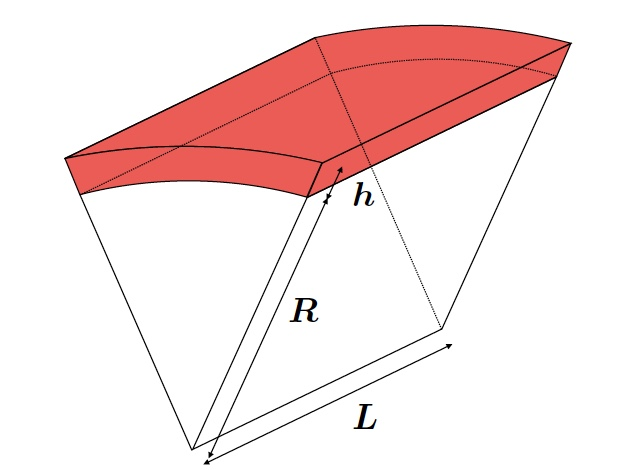
\includegraphics[width=7cm]{scematic_portion_artery.jpg}
\caption{Schematic of a portion of a cylindrical tube.}
\label{fig:solid_}
\end{figure}
\noindent
{\bf Small perturbation assumption}\\
In physiological conditions the wall displacement is small. Therefore the small perturbation assumption, which ties small displacements ${\bf u}$ and strains $\boldsymbol{\epsilon}$, is valid:\\
\begin{equation*}
	\boldsymbol{\epsilon} = \frac{1}{2}(\nabla 	\boldsymbol{u} + \nabla \boldsymbol{u}^\top)
\end{equation*}
\\
{\bf Linear elasticity}\\
We describe the arterial wall in the simplest possible way as an homogeneous, isotropic, isothermal, linear elastic material. Consequently the relation between the Cauchy stress tensor $\boldsymbol{\sigma}$ and the strain tensor $\boldsymbol{\epsilon}$ is given by Hooke's law:
\begin{equation} \label{neo_hook}
	\boldsymbol{\sigma} = \lambda \textrm{tr}(\boldsymbol{\epsilon})\mathbb{I} + 2\mu \boldsymbol{\epsilon} \quad \textrm{or} \quad \boldsymbol{\epsilon} = -\frac{\nu}{E}\textrm{tr}(\boldsymbol{\sigma})\mathbb{I} + \frac{1+\nu}{E}\boldsymbol{\sigma}
\end{equation}
where $\lambda$ and $\mu$ are the Lamé parameters of the wall and $E$ and $\nu$ are respectively the Young's modulus and the Poisson coefficient.\\
\\
{\bf Linear elasticity}\\
The general momentum balance equation for an incompressible material writes:
\begin{equation*}
\rho \frac{\textrm{D}\boldsymbol{v}}{\textrm{D}t} = \rho \boldsymbol{f_v}+\nabla\cdot\boldsymbol{\sigma}
\end{equation*}
where $\rho$ is the density of the material, $\boldsymbol{v}$ is the velocity vector and $\boldsymbol{f_v}$ the vector of volume forces. By introducing non-dimensional variables and using realistic values of the parameters the equation simplifies to the quasi-static equilibrium equation:
\begin{equation*}
\nabla\cdot\boldsymbol{\sigma} = 0
\end{equation*}
\subsubsection{Thin cylinder all law}
Combining these hypothesis, we obtain simplified equations for the displacement of the arterial wall, usually referred to as Lamé equations:
\begin{equation} \label{eq:1}
[\lambda + 2\mu]\nabla(\nabla\cdot\boldsymbol{u})-\mu\nabla\times(\nabla\times\boldsymbol{u}) = 0
\end{equation}
The final step is to provide boundary conditions to equation \ref{eq:1}. We assume that the artery does not deform in the axial direction, or more accurately that the axial displacement is small compared to the length of the artery, and that pressure is the only significant stress applied to the internal and external sides of the artery:
\begin{equation} \label{boundary:2}
  \left\{
      \begin{aligned}
       & \epsilon_{xx} = 0 \\
       & \boldsymbol{\sigma} \cdot \boldsymbol{n} = -p\boldsymbol{n} &\qquad \text{at\quad} r &=R\\
       & \boldsymbol{\sigma} \cdot \boldsymbol{n} = -p_{ext}\boldsymbol{n} &\qquad \text{at\quad} r &=R+h
      \end{aligned}
    \right.
\end{equation}
where $p$ and $p_{ext}$ are respectively the internal and the external fluid pressures. From now on we consider $p_{ext}$ constant\\
\\
{\bf Thick wall}\\
We solve the system \ref{eq:1} by choosing kinetically admissible form for the displacements $\boldsymbol{u}$:
\begin{equation*}
\boldsymbol{u} = rf(r)\boldsymbol{e_r}+g(x)\boldsymbol{e_x}
\end{equation*}
injecting this expression in the system and using the first boundary condition of \ref{boundary:2}, we obtain the expressions for $f$ and $g$:
\begin{equation}
  \left\{
      \begin{aligned}
       & f(r) = a + \frac{b}{r^2} \\
       & g(x) = c
      \end{aligned}
    \right.
\end{equation}
Therefore by using the equations introduced above we have the form of the strain tensor $\boldsymbol{\epsilon}$ and applying the other two boundary conditions we obtain the expression of the stress tensor:
\begin{equation} \label{sigma:4}
  \left\{
      \begin{aligned}
       & \sigma_{rr} = A-\frac{B}{r^2} \\
       & \sigma_{\theta\theta} = A+\frac{B}{r^2} \\
       & \sigma_{xx} = C
      \end{aligned}
    \right.
\end{equation}
and
\begin{equation} \label{sigma:4}
  \left\{
      \begin{aligned}
       & A = p \Bigg[\frac{1}{\big[1+\frac{h}{R}\big]^2} - \frac{p_{ext}}{p}\Bigg] \frac{\big[1+\frac{h}{R}\big]^2}{\big[1+\frac{h}{R}\big]^2 -1} \\
       & B = \Big[1- \frac{p_{ext}}{p}\Big]R^2 \frac{\big[1+\frac{h}{R}\big]^2}{\big[1+\frac{h}{R}\big]^2 -1}\\
       & C = 2\lambda a
      \end{aligned}
    \right.
\end{equation}
\\
{\bf Thin wall}\\
Since we are in the hypothesis of thin wall, the width of this is small compared to the radius of the artery. We therefore introduce the small parameter $\epsilon_w$:
\begin{equation*}
	\epsilon_w = \frac{h}{R_0}
\end{equation*}
and write $r$ and $R$ as:
\begin{equation}
  \left\{
      \begin{aligned}
       & r = R_0[1+\epsilon_w\bar{r}] \\
       & R = R_0[1+\epsilon_w\bar{R}]
      \end{aligned}
    \right.
\end{equation}
We then have, by injecting them in System \ref{sigma:4} an expression for $\sigma_{rr}$ and $\sigma_{\theta\theta}$ which linearized ha the following form:
\begin{equation} \label{sigma:6}
  \left\{
      \begin{aligned}
       & \sigma_{rr} \approx p\Big[[\bar{r}-\bar{R}-1]-\frac{p_{ext}}{p}[\bar{r}-\bar{R}]\Big] \\
       & \sigma_{\theta\theta} \approx \frac{p}{\epsilon_w}\Big[1-\frac{p_{ext}}{p}\Big] \\
      \end{aligned}
    \right.
\end{equation}
These equations indicate that $\sigma_{rr} \ll \sigma_{\theta\theta}$ and since $\sigma_{\theta\theta} \approx p -p_{ext}$, the transmural pressure applied on the arterial wall is balanced only by the tangential stress.\\
\\
Neo-Hooke law \ref{neo_hook} gives us a relation between $\boldsymbol{\sigma}$ and $\boldsymbol{\epsilon}$ and by applying the first boundary condition of System \ref{boundary:2}, we can write:
\begin{equation} \label{eq:sigmaeps}
\sigma_{\theta\theta} = \frac{E}{1-\nu_w^2}\epsilon_{\theta\theta}
\end{equation}
Finally since 
\begin{center}
$\boldsymbol{\epsilon} = $
$\begin{matrix}
\begin{pmatrix}
\partial_ru_r & 0 & 0 \\
0 & \frac{u_r}{r} & 0 \\
0 & 0 & \partial_xu_x \\
\end{pmatrix}
\end{matrix}$
\end{center}
Equation \ref{eq:sigmaeps} rewrites in $r = R$:
\begin{equation}
\sigma_{\theta\theta} = \frac{E}{1-\nu^2_w}\frac{R-R_0}{R_0}
\end{equation}
Combining this equation with the second one of System \ref{sigma:6}, we obtain the linearized thin cylinder wall:
\begin{equation} 
p-p_{ext} = \frac{E}{1-\nu_w^2}\frac{h}{R_0^2}[R-R_0]
\end{equation}
Which is usually written in the more general form above, this describes the arterial wall as a spring of rigidity $K$:
\begin{equation}
p-p_{ext} = K\Big[\sqrt{A}-\sqrt{A_0}\Big] \qquad\textrm{where}\quad K = \frac{E}{1-\nu_w^2}\frac{h\sqrt{\pi}}{A_0}
\end{equation}
\\
From now on, in order to derive the System of equations which couple the fluid and solid problem, we will refer to the following relation:
\begin{equation}\label{eq:Hoop law}
p-p_{ext} = K_1 \big[A-A_0\big] \quad \textrm{where} \quad K_1 = \frac{E}{1-\nu_w^2}\frac{h\sqrt{\pi}}{A_0^{3/2}}
\end{equation}
which is no longer linear in the radius, but in the section of the cylinder. In this way we can derive an analytical solution to which we can compare the numerical one (see Section \ref{sec:solution for small amplitudes}). 
\\
\subsection{Simplified fluid equations}
\subsubsection{Simplifying hypotheses}
{\bf Homogeneous Newtonian fluid}\\
In large arteries, the average size of red blood cells (RBCs) is four order of magnitude smaller than the average vessel size (1 in diameter). Moreover, the average shear rate is high, preventing the aggregation of RBCs. As a first approximation,
we consider that blood is a homogeneous Newtonian fluid.\\
\\
{\bf Incompressible flow}\\
To study the propagation of waves in arteries, we have to take into account the hammer wave phenomenon, generated when a fluid in motion is forced to stop and change direction, which commonly occurs when a valve closes. According to the theory both compressibility of the flow and elasticity of the arterial wall are responsible for the propagation of the water hammer wave. The conservation of mass on a control-volume of compressible fluid in an elastic pipe writes:
\begin{equation}
\frac{\partial}{\partial t}[\rho A]+\frac{\partial}{\partial x}[\rho A U_x] = 0
\end{equation}
which can be rewritten as:
\begin{equation}
\frac{1}{\rho}\frac{D\rho}{Dt}+\frac{1}{A}\frac{DA}{Dt} + \frac{\partial U_x}{\partial x} = 0
\end{equation}
As the fluid is compressible and the wall elastic, both the fluid density $\rho$ and the cross-sectional area A of the tube vary with the fluid pressure $p$. This dependence allow us to write the mass conservation as:
\begin{equation} \label{eq:hammer wave velocity}
\frac{1}{\rho c_{wh}^2}\frac{Dp}{Dt}+\frac{\partial U_x}{\partial x} = 0 \qquad \textrm{where} \qquad \frac{1}{c_{wh}^2} = \frac{1}{\frac{dp}{d\rho}} +\frac{1}{\frac{A}{\rho}\frac{dp}{dA}}
\end{equation}
$c_{wh}^2$ is the water hammer wave speed. We therefore introduce the acoustic wave speed of blood:
\begin{equation}
c_{\rho} = \sqrt{\frac{dp}{d\rho}} = 1.584\times 10^5
\end{equation}
and the elastic wave speed in the large arteries:
\begin{equation} \label{eq:elastic speed wave}
c^2 = \frac{A}{\rho}\frac{dp}{dA} \approx 1 \times 10^2
\end{equation}
Then in equation \ref{eq:hammer wave velocity} we can neglect the term corresponding to acoustic velocity, and conclude that blood flow in large arteries is incompressible.\\
\\
{\bf Axisymmetric flow}\\
In accordance to geometrical assumptions made in Section 1.1, we assume that blood flow is axisymmetric ($\partial_\theta = 0$) and that:
\begin{equation}
  \left\{
      \begin{aligned}
       & \frac{\partial u_x}{\partial r} \bigg|_{r=0} = 0\\
       & u_r \big|_{r=0}=0\\
       & u_\theta =0
      \end{aligned}
    \right.
\end{equation}
{\bf Long wavelength}\\
The average radius in large arteries is $R_0 \approx 1$, the pulse wave speed $c \approx 10^2$ and the heart ejection period $T \approx 1$. The wavelength of the pulse wave is then $ \lambda = cT \approx 10^2$. We can therefore introduce a small parameter $\epsilon_\lambda$, called the long wave parameter:
\begin{equation} \label{eq:long wave hypothesis}
\epsilon_\lambda = \frac{R_0}{\lambda} \ll 1
\end{equation}
\subsubsection{The reduced Navier-Stokes-Prandtl model}
These hypothesis leas us to describe the blood flow in an artery with the incompressible axisymmetric Navier-Stokes for homogeneous Newtonian fluid:
\begin{equation} \label{eq:Navier-Stokes}
  \left\{
      \begin{aligned}
       & \frac{1}{r}\frac{\partial}{\partial r}[ru_r]+\frac{\partial u_x}{\partial x}\\
       & \frac{\partial u_r}{\partial t}+u_r\frac{\partial u_r}{\partial r}+u_x\frac{\partial u_r}{\partial x} = -\frac{1}{\rho}\frac{\partial p}{\partial r}+\nu \Bigg[\frac{1}{r}\frac{\partial}{\partial r}\Bigg[r \frac{\partial u_r}{\partial r}\Bigg] - \frac{u_r}{r^2} + \frac{\partial^2 u_r}{\partial x^2}\Bigg]\\
       & \frac{\partial u_x}{\partial t}+u_r\frac{\partial u_x}{\partial r}+u_x\frac{\partial u_x}{\partial x} = -\frac{1}{\rho}\frac{\partial p}{\partial x}+\nu \Bigg[\frac{1}{r}\frac{\partial}{\partial r}\Bigg[r \frac{\partial u_x}{\partial r}\Bigg] + \frac{\partial^2 u_x}{\partial x^2}\Bigg]
      \end{aligned}
    \right.
\end{equation}
where $\rho$ is the density of blood, $\nu$ the kinematic viscosity of blood, $p$ the fluid pressure and $\boldsymbol{u} = [u_r, u_\theta, u_x]^T$ the fluid velocity vector. The system is completed by the following material interface and axisymmetric conditions for a viscous fluid:
\begin{equation}
  \left\{
      \begin{aligned}
       & u_r = \frac{\partial R}{\partial t}+ u_x\frac{\partial R}{\partial x} &\qquad \textrm{in}\quad r = R\\
       & u_x = 0 &\qquad \textrm{in}\quad r = R\\
       & \frac{\partial u_x}{\partial r} \Bigg|_{r = 0} = 0 \\
       & u_r \big|_{r=0}=0\\
       & u_\theta =0
      \end{aligned}
    \right.
\end{equation}
To asses the importance of each term in System \ref{eq:Navier-Stokes}, we introduce non-dimensional variables and their respective orders of magnitude.
\begin{table}[h!]
\centering
\scalebox{0.9}{%
 \begin{tabular}{||c c c c c c c c||}
 \hline
 \- & \- & $t = \frac{\lambda}{c}\bar{t}$ & $ r = R_0\bar{r}$ & $x = \lambda\bar{x}$ & $u_r = U_r\bar{u_r}$ & $u_x = U_x\bar{u_x}$ & $p = p_0 + \Pi \tilde{p} $ \\ [0.5ex] 
 \hline
  $ \rho = 1$ & $\nu = 10^{-2}$ & $\frac{\lambda}{c} = 1$ & $R_0 = 1$ & $\lambda = 10^2$ & \- & $0\leq U_x\leq100$ &\-\\ [0.5ex]
  \hline 
 \end{tabular}}
\end{table}
Then by injecting the non-dimensional variables in System \ref{eq:Navier-Stokes} and applying the principle of least degeneracy to retain the leading order terms, from the first equation of the system we have:
\begin{equation}
U_r = \epsilon_\lambda U_x
\end{equation}
Using the long wave hypothesis, we have $U_r \ll U_x$, this means that $x$-direction is the main flow direction. From experience, we know that viscous and nonlinear effects are small in the large arteries, then the least degeneracy principle states that the pressure gradient must balance the unsteady inertial term in the last equation of System \ref{eq:Navier-Stokes}, which gives:
\begin{equation}
\Pi = \rho U_x c
\end{equation}
Finally, by introducing the Shapiro number, which characterizes the importance of nonlinear effects (see Section \ref{sec:shapiro}):
\begin{equation} \label{eq:shapiro}
Sh = \frac{U_x}{c}
\end{equation}
and the Womersley number:
\begin{equation}
\alpha = R_0 \sqrt{\frac{\omega}{\nu}}
\end{equation}
describing the competition between pulsatile and viscous effects and using the long wave hypothesis, the system reduces to what we refer to as redued Navier-Stokes-Prandtkìl equations (RNSP):
\begin{mdframed}[backgroundcolor=white!20] 
\begin{equation} \label{eq:RNSP}
  \left\{
      \begin{aligned}
       & \frac{1}{\bar{r}}\frac{\partial}{\partial \bar{r}}[\bar{r}\bar{u_r}]+\frac{\partial \bar{u_x}}{\partial \bar{x}} = 0\\
       & \frac{\partial \bar{u_x}}{\partial \bar{t}} + S_h\Bigg[\bar{u_r}\frac{\partial \bar{u_x}}{\partial \bar{r}} + \bar{u_x}\frac{\partial \bar{u_x}}{\partial\bar{x}}\Bigg] = -\frac{\partial \tilde{p}}{\partial\bar{x}} + \frac{1}{\alpha^2}\Bigg[\frac{1}{\bar{r}}\frac{\partial}{\partial \bar{r}}\Bigg[\bar{r}\frac{\partial \bar{u_x}}{\partial \bar{r}}\Bigg]\Bigg]  \\
       & \frac{1}{\rho}\tilde{p}(\bar{x}, \bar{r}, \bar{t}) = \tilde{p}(\bar{x}, \bar{t}) \\
      \end{aligned}
    \right.
\end{equation}
\end{mdframed}
\subsection{One-dimensional equations}
In order to derive an efficient coupling of the fluid and solid problem, we integrate the System \ref{eq:RNSP} over the cross sectional area. We define $A$ and $Q$ as the cross-sectional area and the axial flow rate respectively:
\begin{equation}
A = 2\pi\int_0^R r\textrm{d}r, \qquad Q = 2\pi\int_0^R u_xr\textrm{d}r  
\end{equation}
as well as $\psi$, the non-linear shape factor, and $\tau_{rx}$ the wall shear stress (WSS):
\begin{equation}
\psi = 2\pi\frac{A}{Q^2}\int_0^R ru_x^2\textrm{d}r, \qquad \tau_{rx} = 2\pi\frac{\partial u_x}{\partial r}\Big|_{r=R}
\end{equation}
Then the system writes:
\begin{equation}\label{eq:system avant final}
  \left\{
      \begin{aligned}
       & \frac{\partial A}{\partial t} + \frac{\partial Q}{\partial x} = 0\\
       &  \frac{\partial Q}{\partial t} +\frac{\partial}{\partial x}\Bigg[\psi\frac{Q^2}{A}\Bigg]+\frac{A}{\rho}\frac{\partial p}{\partial x} = \frac{2\pi R}{\rho} \tau_{rx} \\
      \end{aligned}
    \right.
\end{equation}
In order to close the problem we have to express $\psi$ and $\tau_{rx}$ in terms of the flow rate $Q$ and the cross-sectional area $A$, which will be done making some assumption on the shape of the axial velocity. One-dimensional closure hypothesis suggest that we may write the axial velocity $u_x$ as:
\begin{equation}
u_x = \phi\Big(\frac{r}{R}\Big)U
\end{equation}
where $U = Q/A$ is the averaged velocity and $\phi$ is the dimensionless shape profile.\\
A classical approach consist in using the power-law velocity profile:
\begin{equation}
\phi = \frac{\xi+2}{\xi} \Big[1-\bar{r}^\xi\Big]
\end{equation}
for which we have:
\begin{equation} \label{eq:power law}
  \left\{
      \begin{aligned}
       & \psi = 1+\frac{1}{1+\xi}\\
       &  \frac{\textrm{d}\phi}{\textrm{d} \bar{r}}\Bigg|_{\bar{r}=1} = -[2+\xi] \\
      \end{aligned}
    \right.
\end{equation}
These closure relations stem from an $ad$ $hoc$ expression for the shape of velocity profile designed to match the no-slip condition $u_x = 0$, the axisymmetric condition $\textrm{d}_{\bar{r}}\phi|_{\bar{r}= 0} = 0$ and the Poiseuille velocity profile for $\xi = 2$.
Despite the analysis, we set $\psi = 1$ and use the second relation of System \ref{eq:power law}, then \ref{eq:system avant final} rewrites:
\begin{equation} \label{eq:final system with pressure}
  \left\{
      \begin{aligned}
       & \frac{\partial A}{\partial t} + \frac{\partial Q}{\partial x} = 0\\
       &  \frac{\partial Q}{\partial t} +\frac{\partial}{\partial x}\Bigg[\frac{Q^2}{A}\Bigg]+\frac{A}{\rho}\frac{\partial p}{\partial x} = -C_f \frac{Q}{A} \\
      \end{aligned}
    \right.
\end{equation}
where $C_f = 2\pi\nu[2+\xi]$ is the friction coefficient.\\
Finally, using the wall law for pressure \ref{eq:Hoop law}, the System \ref{eq:final system with pressure} becomes:
\begin{mdframed}
\begin{equation} \label{eq:final dimensional system}
  \left\{
      \begin{aligned}
       & \frac{\partial A}{\partial t} + \frac{\partial Q}{\partial x} = 0\\
       &  \frac{\partial Q}{\partial t} +\frac{\partial}{\partial x}\Bigg[\frac{Q^2}{A}+\frac{K}{2\rho}A^2\Bigg] = -C_f \frac{Q}{A} \\
      \end{aligned}
    \right.
\end{equation}
\end{mdframed}


\newpage
\section{Hyper-elastic laws}
\label{Hyper-elastic laws}
In order to discuss about hyperelastic laws, we make a brief recap of finite deformation theory, introducing the deformations gradient, and the Cauchy and Piola stress tensors.\\
\subsection{Finite theroy}
{\bf Deformation gradient}\\
The deformation gradient is defined by:
\begin{equation}
F_{ij}  = \frac{\partial x_i}{\partial X_j}
\end{equation}
and the transformation of a length in the reference state $\mathbf{dX}$ into the deformed state $\mathbf{dx}$ is given by: 
\begin{equation} % 
d x_i = F_{ij}  d X_j 
\end{equation}
\\
{\bf Deformation tensor}\\
Since a pure rotation  not induce any stres in a deformable body, it is often convenient to use rotation-independent measures. Most known is the right Cauchy-Green deformation tensor  ($\mathbf{F}$ is at the right) or Green's deformation tensor $\mathbf{C}$,
\begin{align} % requires amsmath; align* for no eq. number
\mathbf{C} = \mathbf{F}^T \mathbf{F} \\
C_{ij}  = F_{ki}  F_{kj}  \nonumber
\end{align}
The Cauchy-Green tensor gives us the square of local change in distances due to deformation.\\
The invariants of ${\mathbf  {C}}$ are often used in the expressions for strain energy density functions. 

\begin{align*} % requires amsmath; align* for no eq. number
I_1 = tr({\mathbf  {C}}) = \lambda^2_1+ \lambda^2_2+ \lambda^2_3 \\
I_2 =  \lambda^2_1 \lambda^2_2 +  \lambda^2_2 \lambda^2_3 +  \lambda^2_3  \lambda^2_1 \\
I_3 =  det({\mathbf  {C}}) = \lambda^2_1 \lambda^2_2 \lambda^2_3
\end{align*}
where  $\lambda_{i}$ are stretch ratios for the unit fibers that are initially oriented along the directions of three axis in the coordinate systems.\\
\\
{\bf Cauchy and Piola stress tensors}\\
Given a surface on the reference $dS$ and actual $ds$ configurations from the Cauchy stress theorem we have
\begin{equation} 
\mathbf{\sigma} \mathbf{n} dS = \mathbf{P} \mathbf{N} ds 
\end{equation}
where $\mathbf{\sigma}$ and $\mathbf{n}$ are respectively the stress (Cauchy) tensor and the normal to the surface element for the reference configuration and $\mathbf{P}$ (Piola stress), $\mathbf{N}$ the same for the actual one.
Using the Nason's theorem we found
\begin{equation} 
\mathbf{\sigma} = J^{-1} \mathbf{P} \mathbf{F}^{T}
\end{equation}
where J is the determinant of $\mathbf{F}$.\\
\subsection{Hyperelastic laws}
A hyperelastic material supposes the existence of a function which is denoted by the Helmholtz free energy per unit reference volume $\Psi$. This energy  is also known as strain energy density or the strain energy function. In hyperelastic materials, the strain energy function  is only dependent on the deformation gradient $\mathbf{F}$, $\Psi = \Psi (\mathbf{F})$.
Since these materials do not dissipate energy, for any deformation rate $\dot{F}$ stress power and variation of the internal energy $\Psi$ must coincide:
\begin{equation}
\mathbf{P}\cdot \dot{\mathbf{F}} = \frac{\partial \Psi}{\partial \mathbf{F}} \cdot \dot{\mathbf{F}} \quad \Rightarrow \quad \mathbf{P} = \frac{\partial \Psi}{\partial \mathbf{F}} 
\end{equation} 
\\
{\bf Constitutive relations}\\
As long as $\mathbf{F}$, $\mathbf{C}$ and $\mathbf{B}$ have the same spectral representation, i.e. they have the same invariants we can write $\Psi(\mathbf{F}) = \Psi(\mathbf{C}) = \Psi( \mathbf{B})$ or more precisely in terms of the principal stretches, $\Psi(\lambda_1,\lambda_2,\lambda_3)$.

\noindent
We define the constitutive equations in terms of the principal stretches, as long the strain-energy function is an invariant we can propose
\begin{align} 
\Psi = \Psi(\mathbf{C}) = \Psi(\lambda_1,\lambda_2,\lambda_3)
\end{align} 
The free reference state is $\Psi(1,1,1)=0$. From the  strain-energy function the Cauchy stresses are
\begin{align} 
\sigma_i=  J^{-1} \lambda_i { \partial \Psi \over \partial \lambda_i}
\end{align} 
where $J$ is the volume ratio equal to $\lambda_1 \lambda_2 \lambda_3$. 

\noindent
For incompressible material the motion is characterized by the incompressibility constraint $J=1$ then in order to derive a general equation for hyperelastic material we use
\begin{align} 
\Psi = \Psi(\mathbf{F}) - p(J-1)
\end{align} 
The scalar $p$ is an indeterminate Lagrange multiplier and can be identified as a hydrostatic pressure. Now the 
 Cauchy stresses are
 \begin{align} 
\sigma_i=  -p +  \lambda_i { \partial \Psi \over  \partial \lambda_i}
\end{align} 
therefore knowing $\Psi$  in terms of the principal stretches $ \lambda_i$ we can compute the Cauchy tensor directly.\\
\\
{\bf General law}\\
 A very general kind of Hyperelastic law is due to Odgen 
 \begin{equation}
 \Psi = \sum_p {\mu_p \over \alpha_p } (  \lambda^{\alpha_p}_1+ \lambda^{\alpha_p}_2+ \lambda^{\alpha_p}_3 -3 )
 \end{equation}
with the consistency condition:
\begin{equation} 
2 \mu = \sum_p \mu_p \alpha_p
\end{equation}
where $\mu$ is the shear modulus from the linear theory. In this situation we have the Cauchy stress tensor that writes:
 \begin{equation} 
\sigma_i=  -p +  \sum_p \mu_p \lambda_i^{\alpha_p}
\end{equation} 

\subsection{Deformable tubes: stresses and pressure}
\begin{figure}
\centering
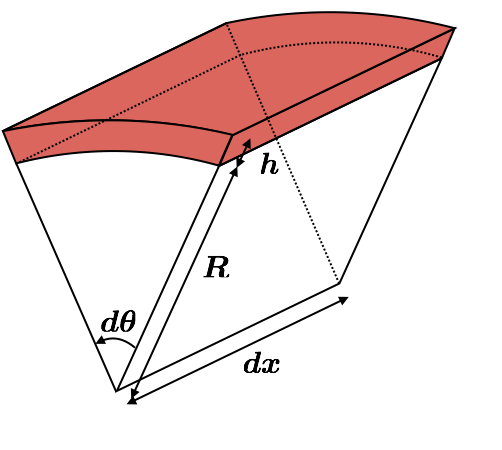
\includegraphics[width=7cm]{solid.png}
\caption{Schema of a cylindrical tube.}
\label{fig:solid}
\end{figure}
We are going to introduce two particular hyperelastic laws, Neo-Hooke and Varga, and, starting from them, we are going to compute the Cauchy stress tensor for a cylindrical deformable tube as schematized in Figure \ref{fig:solid}. Furthermore we will change System \ref{eq:system avant final} in function of the new non-linear relation found for the pressure. \\
\\
{\bf Hypothesis}\\
We have to introduce some hypotheses:
\begin{enumerate}
\item the radial stress is negligible because the thickness of the tube is small compared to the other two directions $h << R$, we are in a case of bi-axial deformation, then $\sigma_3 = 0$ (direction 3 is $r$).
\item We supposed there are not axial displacement then $\lambda_2 \sim 1$ (2 is the $x$ direction).
\item The incompressibility relation $J=1$ says that $\lambda_1 \lambda_2\lambda_3 = 1$ .
\end{enumerate}
Since we do not have deformations along $x$ and $r$, we will focus ourselves on the $\theta$ component of $\sigma$ (tangential deformation), $\sigma_1$.\\
\\
{\bf Pressure relation}\\
 For computing the pressure we have to find the force balance between the pressure difference $p - p_{ext}$ and the stress forces $\sigma_1$ 
 \begin{align}
\Delta p = 2 { H \over R} \sigma_1
 \end{align}
  where $H$ and $R$ are the actual thickness and radius of the elastic tube. As long as the tube inflate the radius increase and the thickness decrease following the incompressibility condition, then:
\begin{align}
H = \lambda_3 h_0 \\
R = \lambda_1 r_0
\end{align}
where $h_0$ and $r_0$ are the equilibrium condition. The pressure relation is now:
\begin{align} \label{eq:pression-stress}
p = 2 { h_0 \over r_0} {\sigma_1 \over \lambda_1^2} + p_{ext}
\end{align}
 giving a non-linear behavior of the pressure for hyperelastic laws.\\
 \\
{\bf Neo-Hookean}\\
The strain energy of this law is given by:
\begin{equation} % requires amsmath; align* for no eq. number
\Psi = {\mu_1 \over 2}(  \lambda^{2}_1+ \lambda^{2}_2+ \lambda^{2}_3 -3 ) = {\mu_1 \over 2} (I_1 -3 )
\end{equation}
with the following Cauchy stress: 
\begin{equation} 
\sigma_i=  -p +  {\mu_1 \over 2}  \lambda_i^{2}
\end{equation}
Thanks to the first hypothesis we can compute the Lagrange multiplier $p$ as: 
\begin{equation} 
p = {\mu_1 \over 2}  \lambda_3^{2}
\end{equation}
and we found the two transverse stress relations: 
\begin{align} 
\sigma_1=  {\mu_1 \over 2} (\lambda_1^{2} - \lambda_1^{-2}\lambda_2^{-2} )\\
\sigma_2=  {\mu_1 \over 2}  (\lambda_2^{2} - \lambda_1^{-2}\lambda_2^{-2} )
\end{align} 
where we have used the relation  $\lambda_1 \lambda_2 \lambda_3 = 1$ to drop off $\lambda_3$. We supposed there are not axial displacement then $\lambda_2 \sim 1$ (2 is the $x$ direction). Taking into account the second and third hypothesis we find:
\begin{equation} 
\sigma_1=  {\mu_1 \over 2} (\lambda_1^{2} - \lambda_1^{-2}).
\end{equation}
 Since $\lambda_1 = \frac{R}{r_0}$ we can rewrite it in function of the areas $\lambda_1^2 = \frac{A}{A_0}$, then:
 \begin{equation}\label{eq:sigma neo hooke}
 \sigma_1 = {\mu_1 \over 2} \Big(\frac{A}{A_0} - \frac{A_0}{A}\Big)
 \end{equation}
 In Equation \ref{eq:pression-stress} we consider $p_{ext}$ constant and substitute $\sigma_1$ with \ref{eq:sigma neo hooke}.
\begin{equation} \label{eq:pressure NH}
p = \frac{\mu h_0}{\sqrt{\pi A_0}}\Bigg(1-\frac{A_0^2}{A^2}\Bigg)
\end{equation}
From now on we will consider $A_0 = 1$. \\
In order to write the equation in the conservative form, we have to express the pressure term as the $x$-derivative of a function of the area $A$. Then we have:
\begin{equation} \label{eq:Neo Hooke pressure law}
\frac{A}{\rho}\frac{\partial p}{\partial x} = 2K_2 \frac{\partial}{\partial x} \Bigg(\frac{1}{A}\Bigg) \quad \textrm{where} \quad K_2 = \frac{\mu h_0}{\rho \sqrt{\pi}}
\end{equation}
furthermore the speed wave is defined as follow:
\begin{equation}\label{eq:speed_NH}
c = \sqrt{\frac{A}{\rho} \frac{\textrm{d}p}{\textrm{d} A}} = \sqrt{2 K_2}\frac{1}{A}
\end{equation}
{\bf Varga}\\
The simplest case of the General Hyperelastic law is given by:
\begin{equation}
\Psi = \mu_1(\lambda_1 + \lambda_2 + \lambda_3 - 3 )
\end{equation}
By making the same passages and using the same hypothesis as we did for Neo-Hooke's law, we obtain the relation for the Cauchy stress:
\begin{equation}
\sigma_1 = \mu_1 (\lambda_1 -\lambda_1^{-1})
\end{equation}
Moreover, thanks to the relation introduced between the deformation along the rayon $\lambda_1$ and the cross-sectional area $A$ and considering $A_0 = 1$, the pressure term will be:
\begin{equation}
p = \frac{2\mu_1 h_0}{r_0} \Bigg({1 \over \lambda_1}-{1 \over \lambda_1^3}\Bigg)  = {4\mu h_0 \over \sqrt{2\pi}} \Bigg(\frac{1}{A^{1/2}}-\frac{1}{A^{3/2}}\Bigg) 
\end{equation}
As well as we did for Neo-Hooke's law, we want to write the pressure in the conservative form, it becomes then:
\begin{equation} \label{eq:Varga pressure law}
\frac{A}{\rho}\frac{\partial p}{\partial x} = K_3 \frac{\partial}{\partial x} \big(A^{1/2}+3 A^{-1/2}\big) \quad \textrm{where} \quad K_3 = {4\mu h_0 \over \rho\sqrt{\pi}}
\end{equation}
with the expression of the elastic speed wave given by \ref{eq:elastic speed wave}, which writes:
\begin{equation} \label{eq:speed_V}
c = \sqrt{\frac{A}{\rho} \frac{\textrm{d}p}{\textrm{d} A}} = \sqrt{K_3}\Big(-\frac{1}{2} A^{-{1\over 2}}+\frac{3}{2}A^{-{3\over 2}}\Big)^{1\over 2}
\end{equation}
%%%%%%%%%%%%%
%%% scrivere della linearizzazione quando la dp/dA <= 0
%%%%%%%%%%%%%

\newpage

\section{Solution for small amplitudes}
\label{sec:solution for small amplitudes}
\subsection{Theory}
Starting from the system \ref{eq:final dimensional system}, we introduce the following non-dimensional variables, in order to rewrite it dimensionless:
\begin{center}
 \begin{tabular}{||c c c c||} 
 \hline
 $ A = A_0\bar{A}$ & $Q = Q_0\bar{Q}$ & $x = L\bar{x}$ & $ t = T_0\bar{t}$ \\ [0.5ex] 
 \hline
 \end{tabular}
\end{center}
From the first equation we can identify a time scale $T_0 = \frac{A_0 L}{Q_0}$ which we call convective time. Moreover, in the second equation, we will substitute the pressure with the previously obtained linear law $p = K(A-A_0)$, which writes:
\begin{equation*}
-\frac{A}{\rho}\frac{\partial p}{\partial x} = -\frac{A}{\rho}K\frac{\partial A}{\partial x} = -\frac{K}{2\rho}\frac{\partial A^2}{\partial x}
\end{equation*}
The final, non-dimensional system is:
\begin{equation}\label{adim-system}
  \left\{
      \begin{aligned}
       & \partial_t A + \partial_x Q = 0\\
       & \partial_t Q + \partial_x (\frac{Q^2}{A} + \epsilon_1 A^2) = -\epsilon_2 \frac{Q}{A}
      \end{aligned}
    \right.
\end{equation}\\
where $\epsilon_1 = \frac{K}{2\rho}\frac{A_0^2 T_0}{LQ_0}$ and $\epsilon_2 = \frac{8\pi \nu T_0}{A_0}$, to find this we set the parameter $\xi = 2$ .\\
\linebreak
Since we look for solutions of small amplitudes, we make the hypothesis $A = A_0+A$ and $Q = Q_0 + Q$, where $A_0 = 1$ and $Q_0 = 0$, therefore the linearization of the system gives:
\begin{equation*}
  \left\{
      \begin{aligned}
       & \partial_t A + \partial_x Q = 0\\
       & \partial_t Q + \partial_x (2\epsilon_1 A) = -\epsilon_2 Q
      \end{aligned}
    \right.
\end{equation*}\\
By deriving the first equation by $x$ and the second by $t$ we obtain the wave equation:
\begin{equation*}
\partial_{tt}Q-2\epsilon_1\partial_{xx}Q=-\epsilon_2\partial_tQ
\end{equation*}
Finally, imposing $Q= \hat{Q}e^{i(kx-\omega t)}$ where $k \in \mathbb{C}$, $k = k_r + ik_i$, then the we have the system for real and imaginary part:
\begin{equation*}
	\left\{
      \begin{aligned}
       & -\omega^2+2\epsilon_1(k_r^2-k_i^2) = 0\\
       & 4\epsilon_1k_rk_i - \omega\epsilon = 0
      \end{aligned}
    \right.
\end{equation*}
If we suppose $k_i \ll k_r$, then $k_r \simeq \frac{1}{\sqrt[]{2\epsilon_1}}\omega$ and $k_i \simeq \frac{\epsilon_2}{2}\frac{1}{\sqrt[]{2\epsilon_1}}$, by taking $\epsilon_1 = \frac{1}{2}$, the condition that has to be satisfied is $\epsilon_2 \ll 2\omega$.\\
\\
Then, the problem \ref{adim-system} with initial conditions
\begin{equation*}
	\left\{
      \begin{aligned}
       & Q = 0 & \forall x\\
       & A = 1 & \forall x
      \end{aligned}
    \right.
\end{equation*}
for small amplitudes, has solution:
\begin{equation}
Q(x,t) = Re\big(e^{ik_rw-\omega t}\big)e^{-k_ix}
\end{equation} 
In the next figure we plotted the impulse in different time steps, we can observe the exponential decreasing of the amplitude as time passes.
\begin{figure}[H]
  \centering
    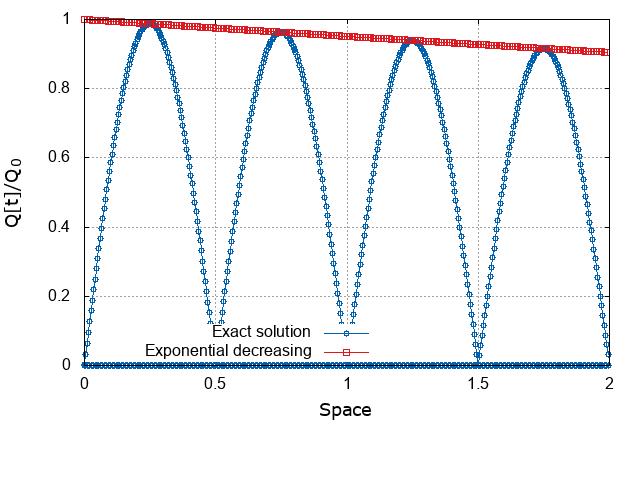
\includegraphics[width=12cm]{Exact_exponential.png}
    \caption{Exact solution $Q(t)$}
\end{figure}


\newpage 
\section{Numeric methods}
\label{sec:numerical}
In this section we present the general form of systems of conservation laws and following the numerical method used to solve the hyperbolic system. 

\subsection{Conservative laws}
The general form of a system of conservation laws is:
\begin{equation} \label{eq:conservative law general}
\frac{\partial \boldsymbol{u}}{\partial t} +  \frac{\partial \boldsymbol{f}(\boldsymbol{u})}{\partial x}  = \boldsymbol{0}
\end{equation}
where $\boldsymbol{f}(\boldsymbol{u})$ are called the flux-functions. One says that System \ref{eq:conservative law general} is written in \textit{conservative form}.
Formally, the System \ref{eq:conservative law general} expresses the conservation of the quantity $\boldsymbol{u}$. In fact let $D$ be an arbitrary domain, and let $\boldsymbol{n}$ be the outward unit normal to the boundary $\partial D$ of the domain. Then, it follows from \ref{eq:conservative law general} that:
\begin{equation}
\frac{d}{dt} \int_D \boldsymbol{u}d\boldsymbol{x} + \int_{\partial D} \boldsymbol{f}(\boldsymbol{u})\boldsymbol{n} dS = \boldsymbol{0}
\end{equation}
This balance equation has now a natural meaning: the time variation of $\int_D \boldsymbol{u}d\boldsymbol{x}$ is equal to the losses through the boundary $\partial D$.\\
For all $j = 1,...,d$ we define the Jacobian matrix of $\boldsymbol{f}$:
\begin{equation}\label{eq:matrix}
\boldsymbol{A}(\boldsymbol{u}) = \frac{\partial \boldsymbol f(\boldsymbol{u})}{\partial \boldsymbol{u}}
\end{equation}
Then, the System \ref{eq:conservative law general} rewrites:
\begin{equation} \label{eq:hyperbolic}
\frac{\partial \boldsymbol{u}}{\partial t} +  \boldsymbol{A}(\boldsymbol{u}) \frac{\partial\boldsymbol{u}}{\partial x}  = \boldsymbol{0}
\end{equation}
By defining the eigenvalus $\lambda_i$ where $i = 1,...,dim(A)$ of the matrix as the solutions of the system:
\begin{equation}
|\boldsymbol{A} - \lambda \mathbb{I}| =0
\end{equation}
and their respective right eigenvectors:
\begin{equation}
\boldsymbol{A}\boldsymbol{r}_i = \lambda_i\boldsymbol{r}_i
\end{equation}
then the System \ref{eq:hyperbolic} is called \textit{hyperbolic} if $\lambda_i \in \mathbb{R} \quad \forall i$, in addition if all the eigenvalues are distinct, the System \ref{eq:hyperbolic} is \textit{strictly hyperbolic}.\\
\\
{\bf Linear advection equation}\\
We now consider the 1D model, where in general $u = u(x,t)$ represents the density or the concentration of a physical quantity $Q$ and $q(u)$ is its flux function. Then the equation is of the form:
\begin{equation} \label{eq:conservation salsa}
u_t + q(u)_x = 0, \qquad x \in \mathbb{R}, t > 0
\end{equation}
As we said before, a conservation law states that, without sources or sinks, the rate of change of $Q$ in the interior of a domain $[x_1,x_2]$ is determined by the net flux through the end points of the interval. Then the law translates int the equation:
\begin{equation}
\frac{d}{dt} \int_{x_1}^{x_2} u(x,t)dx = -q(u(x_2,t))+q(u(x_1,t))
\end{equation}
where we assume that $q > 0$ ($q < 0$) for a flux along the positive (negative) direction of the $x$ axes. From here we can find \ref{eq:conservation salsa}. At this point we have to establish a constitutive relation for $q$, since we consider the linear advection equation we choose a for $q$ a linear function of $u$, namely:
\begin{equation*}
q(u) = au
\end{equation*}
where $a$ is constant. \\
The result is a \textit{pure transport} model, in which the vector $a\boldsymbol{i}$ is the advection speed.\\
\\
The pure transport equation writes:
\begin{equation} \label{eq:linear advection}
u_t +a u_x = 0
\end{equation}
Introducing the vector $\boldsymbol{a} = a \boldsymbol{i} + \boldsymbol{j}$, then Equation \ref{eq:linear advection} can be rewritten in the form:
\begin{equation}
\nabla u \cdot \boldsymbol{a} = 0
\end{equation}
pointing out the orthogonality of $\nabla u$ and $\boldsymbol{a}$. But $\nabla u$ is orthogonal to the level lines of $u$, along which $u$ is constant. Therefore the level lines of $u$ are straight lines parallel to  $\boldsymbol{a}$:
\begin{equation*}
x = at+x_0
\end{equation*}
By computing $u$ along $x = at+x_0$, we find that $u$ is constant along the characteristic lines.\\
\begin{figure}[H]
  \centering
    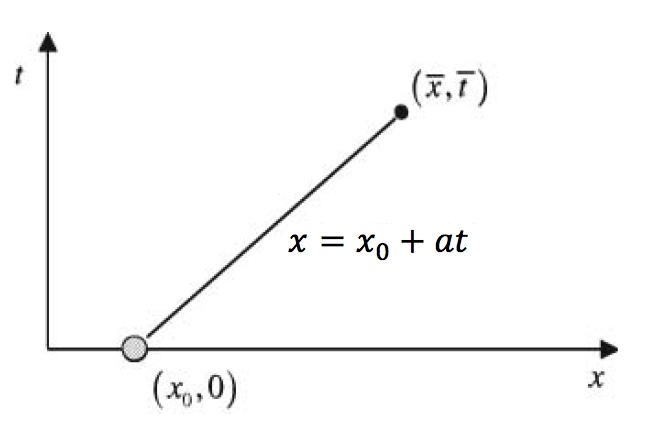
\includegraphics[width=10cm]{char_method.jpg}
    \caption{Characteristic line for the linear transport problem, image taken from \cite{salsa}.}
\end{figure}
If we want to compute the solution at a point $(\bar{x}, \bar{t})$, we take the characteristic line passing through the point and go back in time along this line until the point $(x_0,0)$. If $g(x)$ is the initial profile of $u$ and, knowing that $u$ is constant along the characteristic, then it must be:
\begin{equation*}
u(\bar{x}, \bar{t}) = g(x_0) = g(\bar{x} -a\bar{t})
\end{equation*}
Therefore, the solution of the initial value problem is given by:
\begin{equation} \label{eq:char line solution}
u(x,t) = g(x-at)
\end{equation}
The solution \ref{eq:char line solution} represents a traveling wave, moving with speed $a$ in the positive direction of the $x$ axes.
\begin{figure}[H]
  \centering
    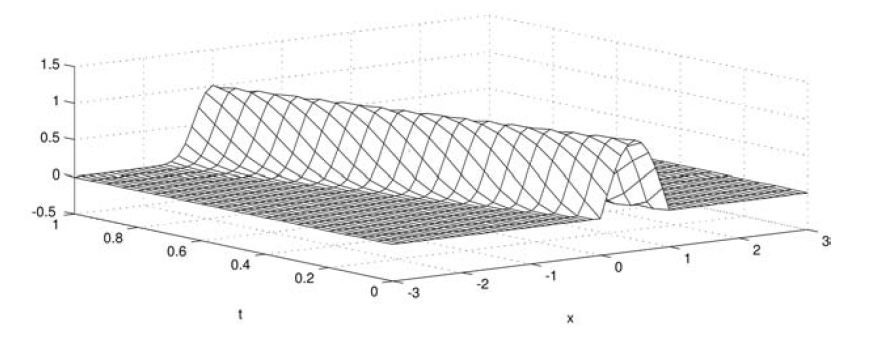
\includegraphics[width=12cm]{Traveling_wave_solution.jpg}
    \caption{Traveling wave solution of the linear transport equation, image taken from \cite{salsa}.}
\end{figure}
\subsection{Conservative method}
Central differences cannot be used to approximate the conservation law, even in the simplest case of linear transport. For linear transport equations, the crucial step in designing an efficient scheme was to upwind it by taking derivatives in the direction of information propagation. For a linear equation with constant coefficient, the direction of information propagation is given by the constant velocity field. For a nonlinear conservation law, the wave speeds depend on the solution itself and can not be determined a priori. Thus, it is not
clear how differences can be upwinded.\\
Another issue is the very nature of finite difference approximations. The key idea underlying finite difference schemes is to replace the derivatives in equations like \ref{eq:conservation salsa} with a finite difference. This procedure requires the solutions to be smooth and the equation to be satisfied point-wise. However, the solutions to the scalar conservation law \ref{eq:conservation salsa} are not necessarily smooth and so the Taylor expansion – essential for replacing derivatives with finite differences – is no longer valid.
\subsubsection{Finite volume method}
The finite volume method in one spatial dimension is based on dividing the
spatial domain into intervals (called finite volumes or cells) making in each
of them an approximation of the integral of the conservative variables. At
each time step these values are updated using approximations of the flux
at the ends of the intervals using the scalar conservation law 
\begin{equation} \label{eq:starting point}
\frac{\partial u}{\partial t} + \frac{\partial f}{\partial x} = 0, \quad u = u(x,t), \quad f = f(u)
\end{equation}
{\bf Integral form}\\
A way to discretize \ref{eq:starting point}, is to divide the spatial
domain into finite volumes and integrate the equation in each cell, transforming
it into an integral form. For simplicity, we will use intervals with equal length $\triangle x$ and take a constant time step $\triangle t$. Thus the
spatial and temporal domains will be:
\begin{align*}
& I_i =\Big[x_{i-{1\over 2}}, x_{i+{1\over 2}}\Big] = \Big[x_i- \frac{\triangle x}{2}, x_i+\frac{\triangle x}{2}\Big] \\
& I_n = [t_n, t_{n+1}] = [n\triangle t, (n+1)\triangle t]
\end{align*}
and the integral in the cell, of Equation \ref{eq:starting point}:
\begin{equation}
\int_{x_{i-{1\over 2}}}^{x_{i+{1\over 2}}} \Bigg[\frac{\partial u}{\partial t} + \frac{\partial f}{\partial x}\Bigg] dx = 0
\end{equation}
becomes:
\begin{equation}\label{integrata}
\int_{x_{i-{1\over 2}}}^{x_{i+{1\over 2}}} \frac{\partial u}{\partial t} dx  + f(u(x_{i+{1\over 2}}))-f(u(x_{i-{1\over 2}})) = 0.
\end{equation}
Since the interval ends $u(x_{i\pm{1\over 2}})$ do not depend on time, we can take the derivative out of the space integral.\\
We define $u_i^n$ as the spatial average of the function $u(x,t)$ in the interval $I_i$, at time $t_n = n\triangle t$, i.e
\begin{equation} \label{media}
u_i^n = \frac{1}{\triangle x} \int_{x_{i-{1\over 2}}}^{x_{i+{1\over 2}}} u(x, t_n)dx
\end{equation}
Integrating Equation\ref{integrata} between $t_n$ and $t_{n+1}$ the time derivative disappears from the first term and we see that the value of $u$ in $I_i$ only changes along time $\triangle t$ due to the value of the flux $f$ at the ends of $I_i$. Then, using \ref{media}, we can write:
\begin{equation}
(u_i^{n+1} - u_i^n)\triangle x + \int_{x_{i-{1\over 2}}}^{x_{i+{1\over 2}}} \Big[f(u(x_{i+{1\over 2}}, t)) - f(u(x_{i-{1\over 2}}, t))\Big] =0
\end{equation}
\begin{figure}[H]
  \centering
    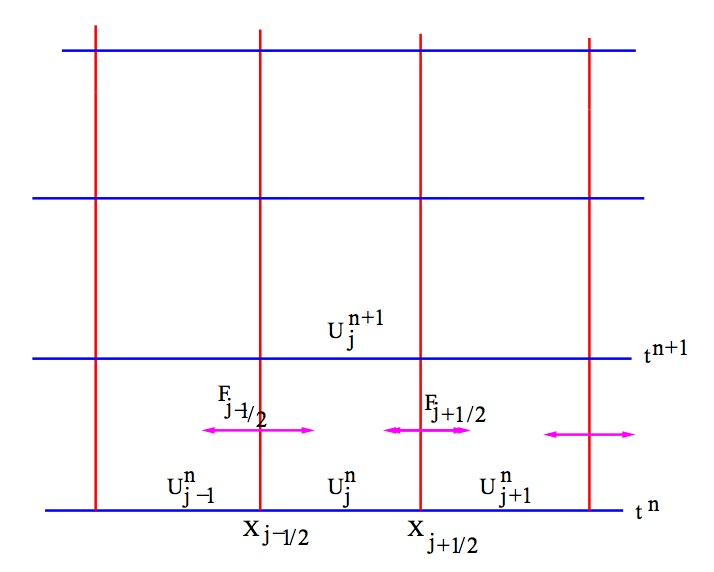
\includegraphics[width=8cm]{grid.jpg}
    \caption{ A typical finite volume grid displaying cell averages and fluxes, image taken from \cite{num_met}.}
    \label{fig:grid}
\end{figure}
\noindent
{\bf Numerical fluxes}\\
In the above expression, the values of the integral of $f$ at points $x_{i\pm {1\over 2}}$ will not be generally known, so we replace them with:
\begin{equation}
f_{i\pm {1\over 2}}^n \approx \frac{1}{\triangle t} \int^{t_{n+1}}_{t_n} f(u(x_{i\pm {1\over 2}},t))dt
\end{equation}
so we get:
\begin{equation} \label{eq:numerical scheme}
u_i^{n+1} = u_i^n -\frac{\triangle t}{\triangle x} \Big(f_{i+ {1\over 2}}^n-f_{i- {1\over 2}}^n\Big) 
\end{equation}
This explicit algorithm allows us to obtain the approximation of $u$ in each cell, at time $t_{n+1}$, from its value in the previous time and the numerical fluxes $f_{i\pm {1\over 2}}^n$ at the ends of the cell.\\
\\
{\bf Rusanov method}\\
The simplest numerical flux to use is the Rusanov flux. This is given by: 
\begin{equation} \label{eq:rusanov}
\boldsymbol{f}_{i+{1\over 2}}^n = {1 \over 2}\big[\boldsymbol{f}(\boldsymbol{u}_i^n) + \boldsymbol{f}(\boldsymbol{u}_{i+1}^n)- \lambda(\boldsymbol{u}_{i+1}^n - \boldsymbol{u}_i^n)\big] 
\end{equation}
Here $\lambda$ is a parameter defined as follow:
\begin{equation}
\lambda = \sup_{u = u_{i+1}, u_{i}} \sup_j |\lambda_j|
\end{equation}
In other words $\lambda$ is the maximum of the absolute eigenvalues of the matrix $\boldsymbol{A}(\boldsymbol{u})$ defined in Equation \ref{eq:matrix}.\\
Taking into account System \ref{adim-system}, vectors $\boldsymbol{u}$ and $\boldsymbol{f}$ are respectively the vector of conservative variables and the vector of
mass and momentum fluxes.\\
\\
In the case of the linear law, the associated matrix is:
\begin{equation}
\boldsymbol{A}(\boldsymbol{u}) = 
\begin{matrix}
\begin{pmatrix}
0 & 1  \\
-{Q^2 \over A^2} + 2\epsilon_1 A & 2{Q \over A} \\
\end{pmatrix}
\end{matrix}
\end{equation}
Then the eigenvalues are given by:
\begin{equation}
\lambda_{1,2} = \frac{Q}{A} \pm \sqrt{2\epsilon_1 A}
\end{equation}
which can be written as the sum of the velocity of the flux and the wave speed:
\begin{equation*}
	\left\{
      \begin{aligned}
       & \lambda_1 = U + c = \frac{Q}{A} + c\\
       & \lambda_1 = U - c = \frac{Q}{A} - c
      \end{aligned}
    \right.
\end{equation*}
By defining:
\begin{equation} \label{eq:H}
H = \frac{Q^2}{A} + \epsilon_1 A^2
\end{equation}
the fluxes are of the form:
\begin{align}
\label{eq:f_a}
& f_{a, i+{1\over 2}} = {1\over 2}\big[(Q_{i} + Q_{i+1}) - \lambda(A_{i+1} - A_i)\big] \\
\label{eq:f_q}
& f_{q, i+{1\over 2}} = {1\over 2}\big[(H_i +H_{i+1}) - \lambda(Q_{i+1} - Q_i)\big]
\end{align}
\vskip 1\baselineskip
\noindent
{\bf Remark on Riemann solvers}\\
In a general Initial Boundary Value Problem:
\begin{equation}\label{sis:IBVP}
	\left\{
      \begin{aligned}
       & \partial_t \boldsymbol{U} + \partial_x \boldsymbol{F}(\boldsymbol{U}) = 0 \qquad 0<x<L \qquad t > 0\\
       & \boldsymbol{U}(x,0) = \boldsymbol{U}^{(0)}(x)\\
       & \boldsymbol{U}(0,t) = \boldsymbol{U}_L(t)\\
       & \boldsymbol{U}(L,t) = \boldsymbol{U}_R(t)\\
      \end{aligned}
    \right.
\end{equation}
is solved by the explicit conservative scheme that we introduced in equation \ref{eq:numerical scheme}. Here we consider the fluxes of Godunov:
\begin{equation}
\boldsymbol{F}_{i+ {1 \over 2}} = \boldsymbol{F}( \boldsymbol{U}_{i+ {1 \over 2}}(0))
\end{equation}
where $\boldsymbol{U}_{i+ {1 \over 2}}(0)$ is the exact similarity solution of the Riemann problem evaluated at $\frac{x}{t} = 0$.\\
Since the vector of the conserved quantity is $n$-dimensional, then there will be $n$ wave families associated to the eigenvalues. In order to make a numerical approximation, we will integrate the first equation of system \ref{sis:IBVP} over the control volume $V = [x_L, x_R] \times [0, T]$, where $x_L < S_L T$ and $x_R > S_R T$, and $S_L$, $S_R$ are respectively the slowest and the fastest signal velocities.\\
\begin{figure}[H]
  \centering
    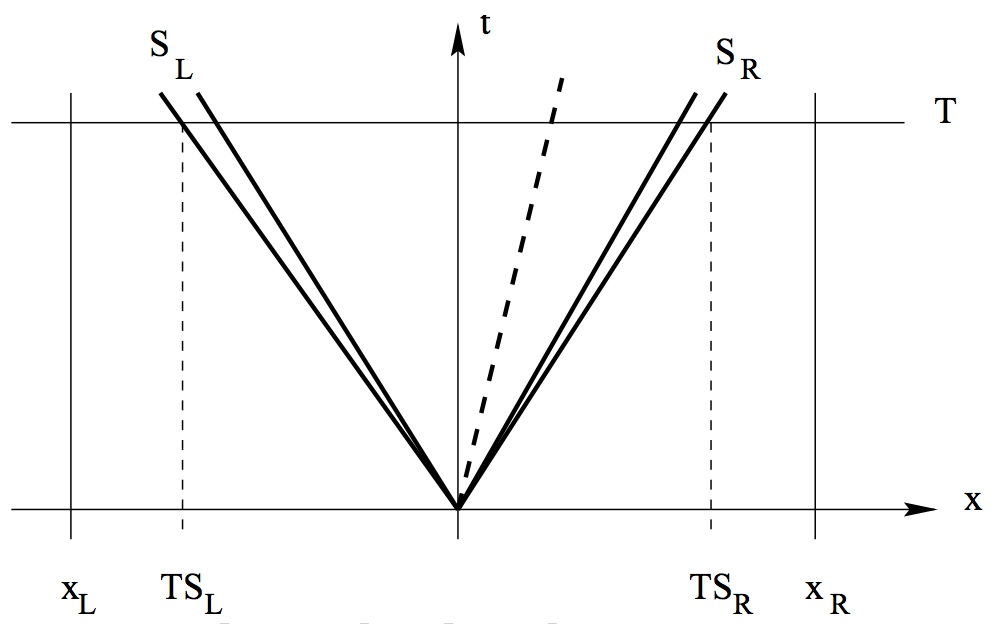
\includegraphics[width=12cm]{ibvp.jpeg}
    \caption{Control volume $[xL, xR] \times [0,T]$ on $x–t$ plane. $S_L$ and $S_R$ are the lowest and fastest signal velocities arising from the solution of the Riemann problem, image taken from \cite{HLLC}.}
    \label{fig:ibvp}
\end{figure}
\noindent
By splitting the volume as in figure \ref{fig:ibvp} and using the consistency condition $F_i = \boldsymbol{F}(\boldsymbol{U}_i)$, we obtain the integral average of the exact solution of the Riemann problem between the slowest and fastest signal:
\begin{equation}\label{eq:UHLL}
\boldsymbol{U}^{HLL} = \frac{S_R \boldsymbol{U}_R - S_L \boldsymbol{U}_L + F_L - F_R}{S_R - S_L}
\end{equation}
The Harten-Lax-van Leer flux for the subsonic case is then defined as:
\begin{equation}\label{eq:Fhll}
\begin{aligned}
& \boldsymbol{F}^{HLL} = \boldsymbol{F}_L + S_L(\boldsymbol{U}^{HLL} - \boldsymbol{U}_L)\\
& \boldsymbol{F}^{HLL} = \boldsymbol{F}_R + S_R(\boldsymbol{U}^{HLL} - \boldsymbol{U}_R)
\end{aligned}
\end{equation}
therefore by injecting equation \ref{eq:UHLL} in one of the definitions \ref{eq:Fhll}, we obtain:
\begin{equation}\label{eq:fhll}
\boldsymbol{F}_{HLL} = \frac{S_R\boldsymbol{F}_L - S_L \boldsymbol{F}_R +S_L S_R (\boldsymbol{U}_R -\boldsymbol{U}_L)}{S_R-S_L}
\end{equation}
There exists many different approximations for the wave speeds, but, since we are considering a one-wave model with a single speed $S^+ > 0$, we can give the exact value to $S_L$ and $S_R$, i.e.: 
\begin{equation*}
S_L = -S^+ \quad \textrm{and} \quad S_R = S^+
\end{equation*}
Then if we substitute these definitions in equation \ref{eq:fhll} we obtain the method of Rusanov described in equation \ref{eq:rusanov}. We can finally conclude that this is an exact method.
\newpage
\section{Results}
\subsection{Comparison between analytic and numeric solution}
The following figures show that the found analytical solution is valid only if the numerical initial impulse has a small amplitude. Indeed, we can observe that in figure \ref{fig:different amplitudes linear} the curve with small initial amplitude, approximate well the analytic one, though we have some discrepancies at the bottom of the figure, due to numerical diffusion, and at the top, which it may be given by the fact that the method is only of order one as we can see in Figure \ref{fig:convergence}.
\begin{figure}[H]
  \centering
    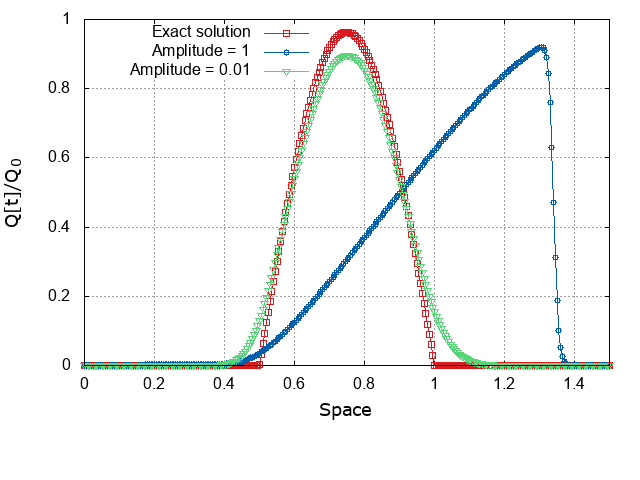
\includegraphics[width=12cm]{exact_linear.png}
    \caption{Comparison between exact solution and numerical solution of the linear law with different initial impulse amplitudes}
    \label{fig:different amplitudes linear}
\end{figure}
\noindent
{\bf Convergence of the scheme}\\
We firstly verify the convergence of the method for small amplitudes (in this case equal to $0.01$). A method converges if for $\triangle x, \triangle t \rightarrow 0$ we have that $u_{num} \rightarrow u_{exact}$. \\
The error norm that we used is computed as follow:
\begin{equation*}
\parallel err \parallel_{L_2} = \frac{1}{\triangle x} \Bigg[\sum_i \parallel u_{exact, i} - u_{num, i} \parallel^2\Bigg]^{1\over 2}
\end{equation*}
Here we took a time-step fixed to $10^{-5}$ and we decreased the space one. We can see in Figure \ref{fig:convergence} that as $\triangle x \rightarrow 0$ the error between the numerical solution and the analytical one tends to $0$, in particular the method is of order one, that means:
\begin{equation*}
\parallel u_{num} - u_{exact} \parallel \sim O(\triangle x)
\end{equation*}
\begin{figure}[H]
  \centering
    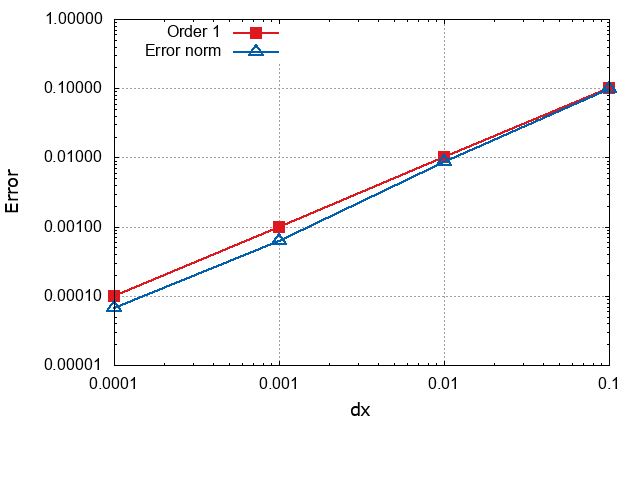
\includegraphics[width=11cm]{Convergence.png}
    \caption{Convergence of the scheme}
    \label{fig:convergence}
\end{figure}
\noindent
{\bf Error in function of the amplitude}\\
We also computed the error between the numerical solution and the analytical one in function of the amplitude. We can notice that by decreasing it the error norm decreases as well, this means that the found analytic solution is well approximated by the linear law $p \sim A$, otherwise it is necessary to introduce non-linear terms.
\begin{figure}[H]
  \centering
    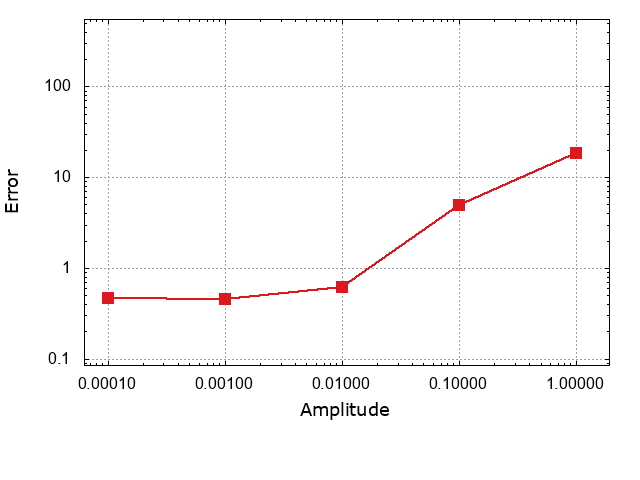
\includegraphics[width=11cm]{error_amplitude.png}
    \caption{$L_2$ error norm in function of the initial impulse amplitude}
    \label{fig:Error_norm}
\end{figure}
\subsection{Non-linear solutions}
We have seen that for small amplitudes, the linear law of pressure in function of the cross-sectional area, is a good approximation of the solution of the problem. But, as soon as the amplitude increases, as shown in Figure \ref{fig:Error_norm}, the error of the numerical solution increases as well.\\
It is for this reason that we will use hyperelastic laws. For this purpose we will start our analysis from System \ref{eq:final dimensional system}.\\
\\
{\bf Neo-Hooke law}\\
In order to obtain the system that will be discretized, we substitute the pressure term in System \ref{eq:final system with pressure} with the relation  \ref{eq:Neo Hooke pressure law}. Then the system rewrites as follow:
\begin{equation}
  \left\{
      \begin{aligned}
       & \frac{\partial A}{\partial t} + \frac{\partial Q}{\partial x} = 0\\
       &  \frac{\partial Q}{\partial t} +\frac{\partial}{\partial x}\Bigg[\frac{Q^2}{A}+2K_2{1 \over A}\Bigg] = -C_f \frac{Q}{A} \\
      \end{aligned}
    \right.
\end{equation}
Proceeding with the same dimensionless parameters introduced in Section \ref{sec:solution for small amplitudes} we obtain the system:
\begin{equation}\label{adim-system NH}
  \left\{
      \begin{aligned}
       & \frac{\partial A}{\partial t} + \frac{\partial Q}{\partial x} = 0\\
       & \frac{\partial Q}{\partial t} + \frac{\partial}{\partial x} \Big(\frac{Q^2}{A} + \epsilon_1 {1 \over A}\Big) = -\epsilon_2 \frac{Q}{A}
      \end{aligned}
    \right.
\end{equation}
where $\epsilon_1 = \frac{2 K_2}{Q_0^2}$ and $\epsilon_2 = \frac{8\pi \nu T_0}{A_0}$.\\
\\
Moreover the numerical fluxes are defined as in Equations \ref{eq:f_a} and \ref{eq:f_q}, we the redefinition of $H$ and of the eigenvalues, more properly of the speed velocity which is defined in Equation \ref{eq:speed_NH}:
\begin{equation}
H = \frac{Q^2}{A} + \epsilon_1 \frac{1}{A}
\end{equation}
{\bf Varga law}\\
As we did for Neo Hooke law, we will start from System \ref{eq:final system with pressure}, replace the pressure gradient with Equation \ref{eq:Varga pressure law} and finally adimensionalize the system here obtained:
\begin{equation}
  \left\{
      \begin{aligned}
       & \frac{\partial A}{\partial t} + \frac{\partial Q}{\partial x} = 0\\
       &  \frac{\partial Q}{\partial t} +\frac{\partial}{\partial x}\Bigg[\frac{Q^2}{A}-K_3 \Bigg(\sqrt{A}+\frac{3}{\sqrt{A}}\Bigg)\Bigg] = -C_f \frac{Q}{A} \\
      \end{aligned}
    \right.
\end{equation}
Then we find:
\begin{equation}
  \left\{
      \begin{aligned}
       & \frac{\partial A}{\partial t} + \frac{\partial Q}{\partial x} = 0\\
       &  \frac{\partial Q}{\partial t} +\frac{\partial}{\partial x}\Bigg[\frac{Q^2}{A}- \epsilon_1\sqrt{A}-\epsilon_2\frac{1}{\sqrt{A}}\Bigg] = \epsilon_3\frac{Q}{A} \\
      \end{aligned}
    \right.
\end{equation}
where $\epsilon_1 = \frac{T_0 K_3 A^{1\over 2}}{L Q_0}$, $\epsilon_2 = \frac{3 K_3 T_0 A_0^{-1 \over 2}}{L Q_0}$ and $\epsilon_3 = \frac{8\pi \nu T_0}{A_0}$.\\
\\
Moreover the numerical fluxes, as well as Neo Hooke's law, are of the form \ref{eq:f_a} and \ref{eq:f_q}, where $c$, which will change the eigenvalues used in the numerical fluxes, is defined in \ref{eq:speed_V} and $H$ as follow:
\begin{equation}
H = \frac{Q^2}{A}-\big(\epsilon_1 A^{1/2}+ \epsilon_2 A^{-1/2}\big)
\end{equation}
\noindent
In the following figure we make a comparison between the non-linear laws, with the exact solution for small amplitudes. We can see that they are similar because by linearizing the hyperelastic laws we should obtain the elastic one, even so, the amplitude does not coincide, both the non-linear laws are around $0.8$, while the exact solution is not much more smaller then $1$. This fact can be explained by the fact that these two solutions are obtain with an initial amplitude of the impulse equal to $0.01$, which probably is not enough small to get the exact linearization.
\begin{figure}[H]
  \centering
    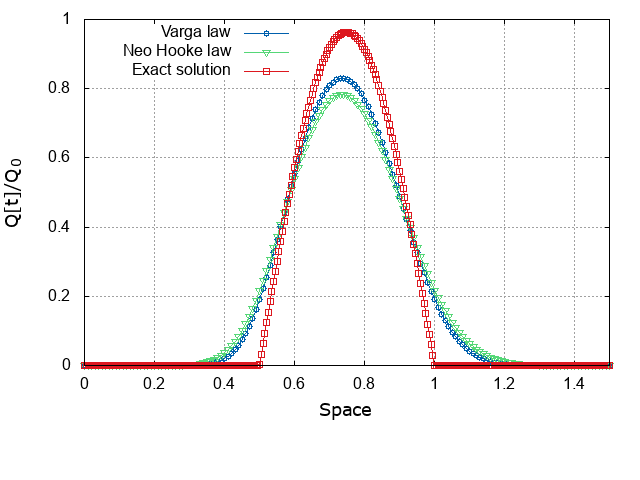
\includegraphics[width=11cm]{exact_hyper_small_amplit.png}
    \caption{Comparison between Neo-Hooke and Varga's laws with the exact solution for small amplitudes}
    \label{fig:V}
\end{figure}
\noindent
Moreover we made a comparison also between the hyperelastic laws and the linear one for big amplitudes. We can observe that the non linear curves maintain the characteristic shape the wave while the one of the elastic law, as we have already seen, cannot approximate well the transmission of the impulse.
\begin{figure}[H]
  \centering
    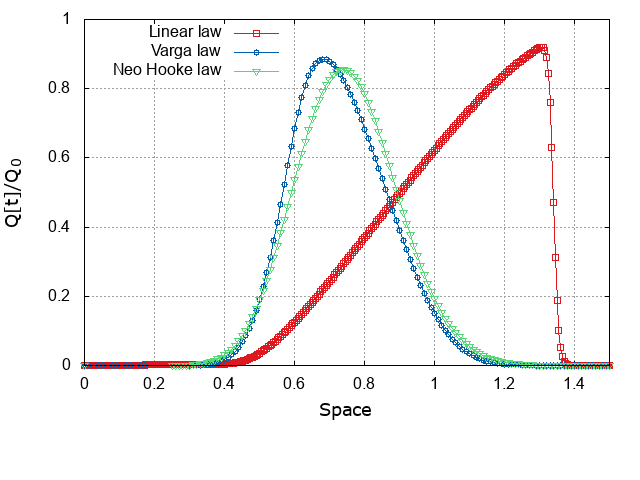
\includegraphics[width=11cm]{Varga_NH_ampli1.png}
    \caption{Comparison between Neo-Hooke and Varga's laws with the linear solution for big amplitudes}
    \label{fig:V}
\end{figure}
%We can notice that, in both Figures \ref{fig:NH} and \ref{fig:V}, the numerical solution has an exponential decreasing. Despite the fact that in the figures, around $Q = 0$, there is always a numerical diffusion, we can state from Figure \ref{fig:hyper-convergence} the two methods converge.
\newpage
\subsection{Subcritical and supercritical cases}
\label{sec:shapiro}
The hyperbolic system
\begin{equation*}
\frac{\partial \boldsymbol{u}}{\partial t} + \frac{\partial \boldsymbol{f}}{\partial x} = 0
\end{equation*}
where
\begin{equation}
\boldsymbol{u} = 
\begin{matrix}
\begin{pmatrix}
A \\
Q \\
\end{pmatrix}
\end{matrix}
\quad \textrm{and} \quad \boldsymbol{f}= 
\begin{matrix}
\begin{pmatrix}
F_A\\
F_Q\\
\end{pmatrix}
\end{matrix}
\end{equation}
is characterized by the Shapiro number $Sh$, defined as:
\begin{equation}
Sh = \Big| \frac{U_x}{c} \Big| = \Big| \frac{1}{c}\frac{Q}{A} \Big|
\end{equation}
Depending on the value of $Sh$, we distinguish two flow regimes, represented respectively by the subcritical velocity domain $\mathbb{U}_{sub}$ and and the supercritical velocity domain $\mathbb{U}_{sup}$. Until now we considered physiological conditions, the flow is subcritical and therefore Shapiro number is $Sh \ll 1$.
\begin{equation*}
	\left\{
      \begin{aligned}
       &  \mathbb{U}_{sub} = \Big\{\frac{Q}{A} \in \mathbb{R} |\quad A > 0,\quad Sh < 1 \Big\}\\
       & \mathbb{U}_{sup} = \Big\{\frac{Q}{A} \in \mathbb{R}|\quad A > 0,\quad Sh > 1 \Big\}
      \end{aligned}
    \right.
\end{equation*}
We will propose two graphs for each law, each one has three curves, the red one represents the deformation of the tube, the other two are the velocities, in particular $U = \frac{Q}{A}$, the velocity of the fluid, (green line) and $c$, the wave speed, the blue line. For the non-linear laws there will be a graph representing also the deformation of the tube in the supercritical case for four different time-steps. The initial condition is given by $Q_0 = const$ until $t = 4s$, then it gets to zero, in particular  $Q_0 = 1$ for Varga, and $Q_0 = 2$ for Neo Hooke. The boundary condition for the cross-sectional area of the tube are a Dirichlet condition at the begin of the tube and a Neumann condition at the end.
%This distinction will be made by taking into account a constant initial flow at the entrance of the tube, for the subcritic case $Q_0 = 0.2$ and for the supercritic $Q_0 = 2$.
\begin{figure}[H]
  \centering
    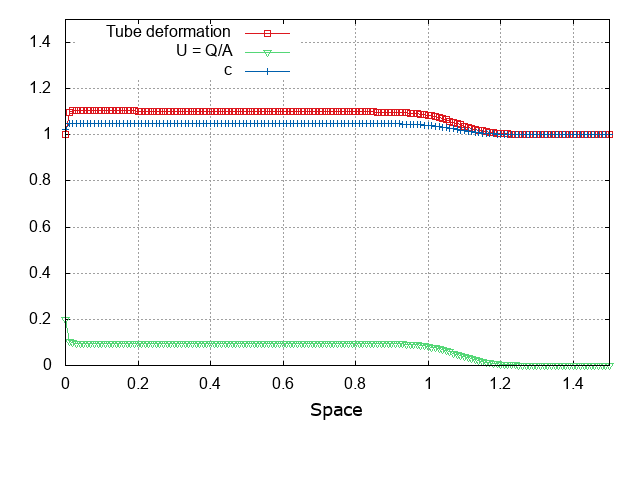
\includegraphics[width=0.7\textwidth]{Linear_Q02_sub.png}
    \caption{Linear, subcritical case}
    \label{fig:Linear_sub}
\end{figure}
\begin{figure}[H]
\centering
    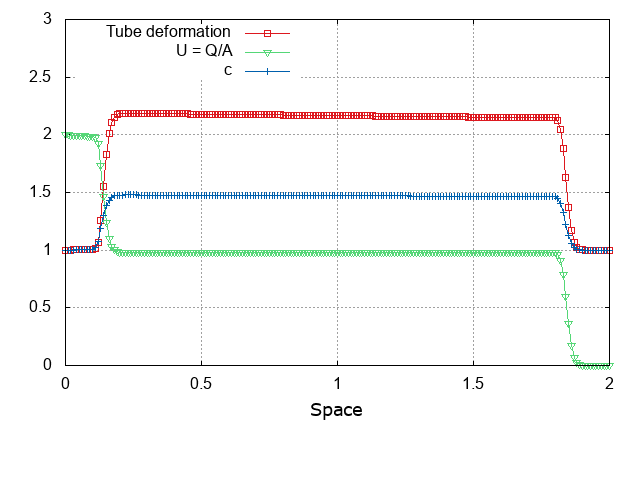
\includegraphics[width=0.7\textwidth]{Linear_Q2_super.png}
    \caption{Linear, supercritical case}
    \label{fig:Linear_super}
\end{figure}
\begin{figure}[H]
  \centering
    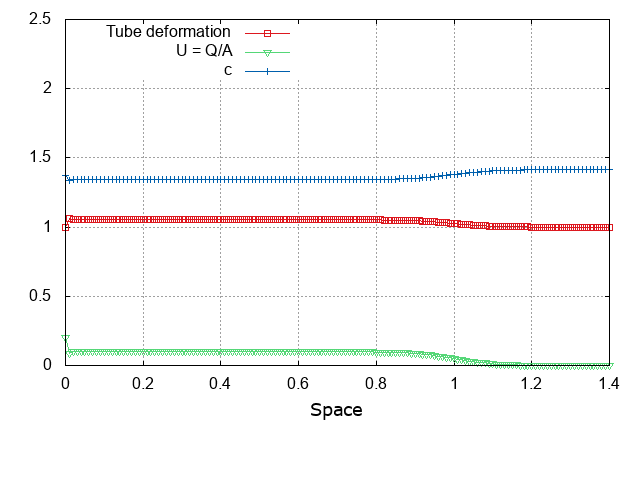
\includegraphics[width=0.7\textwidth]{NH_Q02_sub.png}
    \caption{Neo Hooke, subcritical case}
    \label{fig:NH_sub}
\end{figure}
\begin{figure}[H]
	\centering
    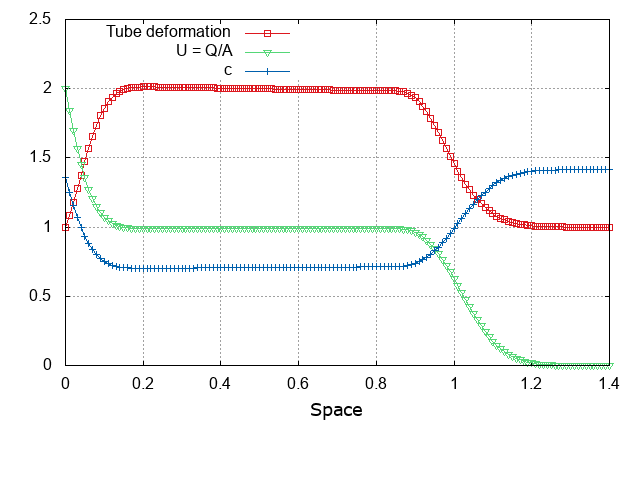
\includegraphics[width=0.7\textwidth]{NH_Q2_super.png}
    \caption{Neo Hooke, supercritical case}
    \label{fig:NH_super}
\end{figure}
\begin{figure}[H]
	\centering
    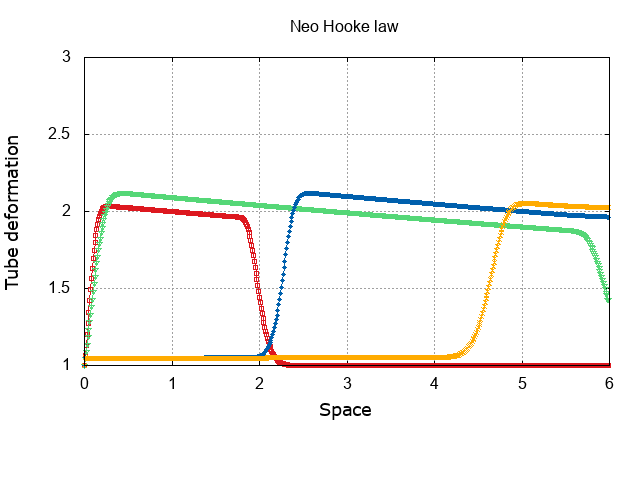
\includegraphics[width=0.7\textwidth]{NH_Q1.png}
    \caption{Neo Hooke, deformation of the tube for four different time steps}
    \label{fig:NH_flux}
\end{figure}
\begin{figure}[H]
  \centering
    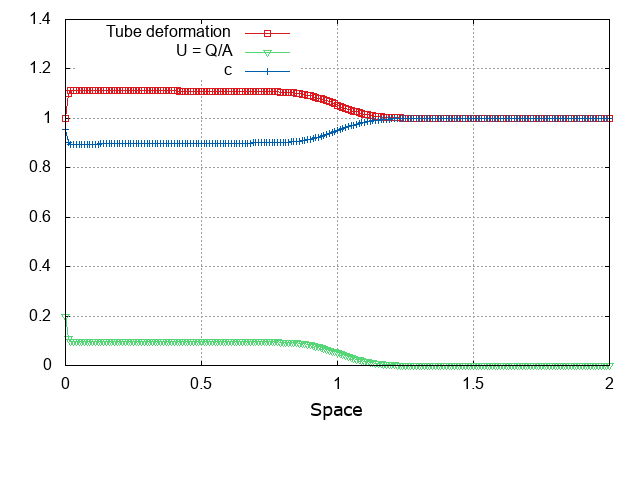
\includegraphics[width=0.7\textwidth]{Varga_Q02_sub.png}
    \caption{Varga, subcritical case}
    \label{fig:Varga_sub}
\end{figure}
\begin{figure}[H]
  \centering
    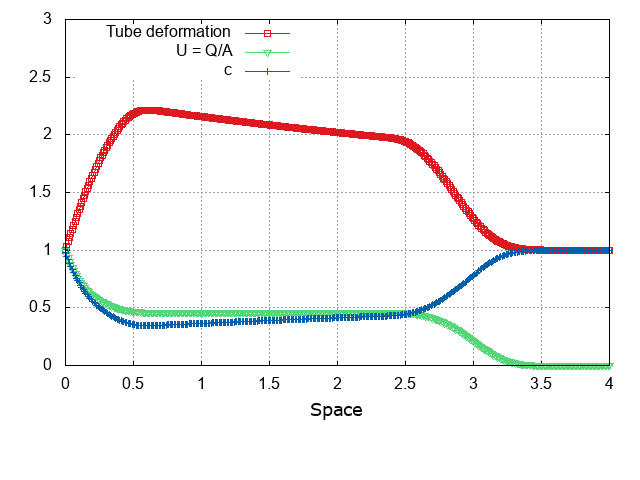
\includegraphics[width=0.7\textwidth]{Varga_Q1_super.png}
    \caption{Varga, supercritical case}
    \label{fig:Varga_super}
\end{figure}
\begin{figure}[H]
	\centering
    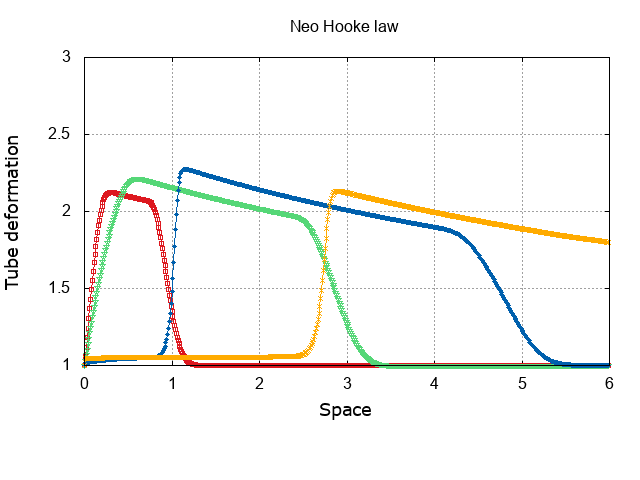
\includegraphics[width=0.7\textwidth]{Varga_Q1.png}
    \caption{Varga, deformation of the tube for four different time steps}
    \label{fig:Varga_flux}
\end{figure}
\noindent
Talking about the subcritical cases, ($Q_0 = 0.2$), we observe that at $x = 0$ we have a small jump, this is due to the fact that we imposed two Dirichlet conditions for both $Q$ and $A$, this choice was made in order to see how velocities evolve.\\
Concerning the supercritical cases we can notice that the discontinuity is more remarked in the graph of the elastic law than in the ones of the non-linear laws, it is not surprising since the difference between the velocity of the fluid and the wave speed is bigger in the linear case then the other two. The jump is significant in any case since, to model the pressure law we have considered the longitudinal stresses small, which induced to neglect the surface tension of the arterial wall and then the term of Laplace pressure:
\begin{equation}
p_L = -\sigma \kappa = -\sigma \frac{A_{xx}}{\big(1+A_x^2\big)^{3/2}}
\end{equation}
\newpage
\section*{Conclusion}
\addcontentsline{toc}{section}{Conclusion}
In this report we have presented the hypothesis for the solid and fluid problem that have allowed us to derive simplified equations for the mechanical response of the arterial wall and for the flow of blood in an axisymmetric artery (RNSP). Equation \ref{eq:Hoop law} and system \ref{eq:RNSP} form the minimal system of equations necessary to accurately describe blood flow in large elastic arteries. \\
\\
Then we introduced the constitutive relations for an elastic material, in particular we described the strain energy function as function of the principal stretches. Then, since we are talking about hyperelastic materials, we introduced the reactive term given by the unknown pressure.  After making some hypothesis, we were able to define the pressure in function of the cross-sectional area, using firstly the strain energy associated to Neo-Hooke and then to Varga. In this way we could rewrite the pressure term in a conservative form in order to use the finite volume method.\\
\\
Moreover, we have been able to find an analytical solution for small amplitudes. It will be used in order to demonstrate the convergence of the method and to verify the domain of validity of the elastic law, indeed it is no more of use when the initial amplitude impulse is no longer small.\\
Talking about numerical approximation, we presented the Rusanov method, used for the simulations, as a particular case of the HLL Riemann solver. In the following section we demonstrate that the scheme is, as we expected of order 1.\\
\\
The results that we obtained are in accordance we the theory. In particular, we have seen that the elastic law is no longer valid as the amplitude increases (see figure \ref{fig:Error_norm}, the validity of the hyperelastic law if linearized (figure \ref{fig:V}), as well as their validity for bigger amplitude of the initial impulse.\\
Finally, talking about the subcritical and supercritical cases, the results are promising as we have to take into account the simplifying hypothesis that we made and the numerical error.
\newpage
\nocite{*}
\bibliographystyle{siam}
\bibliography{biblio}
\end{document}










